\begin{columns}[T]
  \begin{column}{0.55\textwidth}
    \textbf{What is a Credit Score?}
    \begin{itemize}
      \item A base FICO Score is a 3-digit rating from 300 to 850.
      \item Lenders use scores to help estimate the risk of missed payments.
      \item \textbf{Equifax}, \textbf{Experian}, and \textbf{TransUnion} maintain separate credit files.
    \end{itemize}
  \end{column}
  \begin{column}{0.45\textwidth}
    \centering
    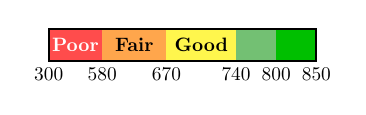
\begin{tikzpicture}[scale=0.68, every node/.style={scale=0.7}]
      % Draw color band for score ranges
      \fill[red!70] (0,0) rectangle (1,0.6);
      \node at (0.5,0.3) {\color{white}\textbf{Poor}};
      \fill[orange!70] (1,0) rectangle (2.2,0.6);
      \node at (1.6,0.3) {\textbf{Fair}};
      \fill[yellow!70] (2.2,0) rectangle (3.5,0.6);
      \node at (2.85,0.3) {\textbf{Good}};
      \fill[green!55!black!55] (3.5,0) rectangle (4.25,0.6);
      \fill[green!75!black] (4.25,0) rectangle (5,0.6);

      \draw[thick] (0,0) rectangle (5,0.6);

      % Labels below
      \node[below] at (0,0) {300};
      \node[below] at (1,0) {580};
      \node[below] at (2.2,0) {670};
      \node[below] at (3.5,0) {740};
      \node[below] at (4.25,0) {800};
      \node[below] at (5,0) {850};
    \end{tikzpicture}
    \vspace{0.5em}

    \small
    \begin{itemize}\small
      \item \textbf{300--579}: Poor
      \item \textbf{580--669}: Fair
      \item \textbf{670--739}: Good
      \item \textbf{740--799}: Very Good
      \item \textbf{800--850}: Exceptional
    \end{itemize}
  \end{column}
\end{columns}
